%=============================================================================
%  SHARED PREAMBLE -- packages, GIC palette, beamer theme and every figure
%  / layout / statistic macro, used by BOTH decks:
%      retailradar_presentation.tex   (full, ~77 pages)
%      retailradar_short.tex          (15-slide cut-down)
%
%  WHY THIS FILE EXISTS.  The short deck is a SELECTION from the full one,
%  not a rewrite, so the two must render identically -- same palette, same
%  fitted figure caps, same SO WHAT strip.  Copying 200 lines of preamble
%  into a second file guarantees they diverge at the first fix applied to
%  only one of them; the measured figure-height comments below are exactly
%  the kind of hard-won detail that gets lost that way.  One source, two
%  \input lines.
%
%  NOT included here, on purpose: \lastedited, \lastcommit and
%  \deckversion.  Each deck states its OWN age and its own last change,
%  because they are edited independently -- a shared date would be a lie on
%  whichever deck was not touched.
%=============================================================================
%------------------------------------------------------------------ packages --
\usepackage[T1]{fontenc}
\usepackage[utf8]{inputenc}
% Latin Modern if the installation has it (it is the nicer face, and every
% full TeX Live / MiKTeX does), silently falling back to Computer Modern if
% not.  Same principle as the figure fallback below: the deck must compile on
% whatever machine it is opened on, and degrade rather than refuse.
\IfFileExists{lmodern.sty}{\usepackage{lmodern}}{}
\usepackage{graphicx}
\usepackage{booktabs}
\usepackage{array}
\usepackage{xcolor}
\usepackage{amsmath}
\usepackage{tikz}
\usepackage{pgffor}
\usetikzlibrary{positioning}

%--------------------------------------------------------------------- theme --
% The GIC institutional palette the dashboard already uses, so the deck and
% the product read as one artefact: navy on white, greys for hierarchy, and
% exactly two accent hues -- one for GET IN, one for GET OUT.  Never vibrant,
% no gradients.
\definecolor{gicnavy}{HTML}{0A1E2E}
\definecolor{gicink}{HTML}{111111}
\definecolor{gicgrey}{HTML}{666666}
\definecolor{giclight}{HTML}{8C8C8C}
\definecolor{gicrule}{HTML}{ECECEC}
\definecolor{gicpanel}{HTML}{F6F7F8}
\definecolor{bullish}{HTML}{1F6F5C}   % deep muted teal-green -- GET IN
\definecolor{bearish}{HTML}{A6413B}   % muted brick          -- GET OUT

\usetheme{default}
\usecolortheme{default}
\setbeamercolor{normal text}{fg=gicink}
\setbeamercolor{frametitle}{fg=gicnavy}
\setbeamercolor{structure}{fg=gicnavy}
\setbeamercolor{itemize item}{fg=gicnavy}
\setbeamercolor{itemize subitem}{fg=gicgrey}
\setbeamercolor{block title}{bg=gicpanel,fg=gicnavy}
\setbeamercolor{block body}{bg=gicpanel,fg=gicink}
\setbeamerfont{frametitle}{size=\large,series=\bfseries}
\setbeamerfont{title}{size=\LARGE,series=\bfseries}
\setbeamertemplate{navigation symbols}{}
\setbeamertemplate{itemize item}{\color{gicnavy}\rule[0.35ex]{0.5em}{0.8pt}}
\setbeamertemplate{itemize subitem}{\color{giclight}\textbullet}
\setbeamertemplate{caption}{\insertcaption}
\setbeamerfont{caption}{size=\scriptsize}
\setbeamercolor{caption}{fg=gicgrey}

% Frame title with the hairline rule underneath -- the one piece of chrome.
% \makeatletter is required because \beamer@leftmargin contains an @, which is
% not a letter in ordinary document code; without it the template expands to
% an undefined control sequence at the first \end{frame}.
\makeatletter
\setbeamertemplate{frametitle}{%
  \vspace{0.6em}%
  \begin{minipage}{\dimexpr\paperwidth-2\beamer@leftmargin\relax}
    \raggedright\usebeamerfont{frametitle}\usebeamercolor[fg]{frametitle}%
    \insertframetitle\par\vspace{0.35em}%
    {\color{gicrule}\hrule height 0.8pt}%
  \end{minipage}\vspace{0.4em}}
\makeatother

% Footer: page number, deck age, and the last commit message -- so nobody
% presents a six-week-old number without knowing it.
\setbeamertemplate{footline}{%
  \hbox{\begin{beamercolorbox}[wd=\paperwidth,ht=2.4ex,dp=1.4ex,
        leftskip=1.2em,rightskip=1.2em]{}%
    {\color{giclight}\scriptsize RetailRadar \textbullet\ \deckversion\
     \textbullet\ last edited \lastedited}%
    \hfill{\color{giclight}\scriptsize\insertframenumber}%
  \end{beamercolorbox}}}

%------------------------------------------------------------------- helpers --
\graphicspath{{../figures/}{../../docs/figures/}{./figures/}}

% \gfig{path}{width fraction}{caption}
% Falls back to a visible placeholder if the PNG has not been exported yet,
% so an incomplete export never blocks a rehearsal.
%
% The height cap is a MACRO, not a literal, for one practical reason: a slide
% carrying a figure plus a caption plus a SO WHAT strip overflows the frame,
% and the fix is always "give the picture less height", never "delete the
% reasoning".  A frame that needs it says \tightfig (or \tighterfig) at the
% top; because a frame is a TeX group the setting reverts on \end{frame}, so
% one slide's squeeze cannot leak into the next.
% \figh{0.41} sets the cap to an exact measured value; \tightfig and
% \tighterfig are just the two named presets.  The exact values in this file
% are not taste -- they were FITTED: compile, read the "Overfull \vbox (Xpt too
% high)" figure out of the log, and take exactly X pt (plus 4pt of slack) off
% the picture.  Which dimension to take it from depends on what governs:
%
%     rendered height  h = min(\figmaxh * \textheight,  width * L * aspect)
%
% so a TALL figure is cap-governed (lower \figh) and a WIDE one is
% width-governed (lower the \gfig width fraction -- lowering the cap on a wide
% figure does nothing at all, which is the trap this comment exists to record).
% Measured on this class: \textheight = 252.07pt, \linewidth = 398.34pt, and
% L = 199.17pt inside a half-width column.
\newcommand{\figmaxh}{0.62}
\newcommand{\figh}[1]{\renewcommand{\figmaxh}{#1}}
\newcommand{\tightfig}{\figh{0.46}}
\newcommand{\tighterfig}{\figh{0.38}}
\newcommand{\gfig}[3]{%
  \IfFileExists{../figures/#1}{%
    \begin{center}
      \includegraphics[width=#2\linewidth,height=\figmaxh\textheight,
                       keepaspectratio]{#1}
    \end{center}
    \ifx\relax#3\relax\else
      {\scriptsize\color{gicgrey}#3\par}\fi}{%
    \begin{center}
      \begin{tikzpicture}
        \draw[gicrule,line width=0.8pt,fill=gicpanel]
          (0,0) rectangle (0.86\linewidth,0.42\textheight);
        \node[align=center,text=giclight,font=\scriptsize]
          at (0.43\linewidth,0.21\textheight)
          % \detokenize because exported filenames contain underscores, which
          % are subscript characters in ordinary text mode and would abort the
          % build with "Missing $ inserted" the moment a figure is absent --
          % i.e. exactly in the situation this fallback exists to survive.
          {figure not yet exported\\
           \texttt{\detokenize{docs/figures/#1}}\\[2pt]
           run \texttt{python tools/export\_figures.py -{}-all}};
      \end{tikzpicture}
    \end{center}
    \ifx\relax#3\relax\else{\scriptsize\color{gicgrey}#3\par}\fi}}

% A caption set UNDER a pair of side-by-side figures, at full slide width.
% Why it exists: a caption inside a half-width column wraps at 199pt, so 30
% words become seven lines, and seven lines of \scriptsize is ~56pt of the
% 252pt text block -- taken straight out of the pictures.  The same words
% across the full width take four.  Used on the dashboard-pair slides, where
% the figures are screenshots and shrinking them any further would make the
% product unreadable.  Same words, half the height.
\newcommand{\figcap}[1]{{\scriptsize\color{gicgrey}#1\par}}

% \pb -- a zero-width place where a long path in code face MAY break.
% \texttt gives TeX no breakpoints whatsoever, so a filename like
% docs/research/nb01_episode_stats.json inside the SO WHAT strip simply ran
% 47pt past the edge of the box.  Shortening the path is not an option: the
% path IS the citation, and the whole provenance argument of this deck rests on
% a reviewer being able to open the file.  So the path stays complete and is
% allowed to wrap instead, at the separators, where a reader's eye expects it.
\newcommand{\pb}{\discretionary{}{}{}}

% \sidefig{path}{caption}{so what} -- figure LEFT, words RIGHT.
%
% Why a second layout exists at all: on a 16:9 slide the text block is 398pt
% wide and 252pt tall, so its own aspect is 0.63.  A figure TALLER than that
% (a square heatmap at 0.81, a full-page screenshot at 0.69) is height-bound
% when stacked above its caption -- it hits the cap long before it runs out of
% width, and the slide ends up with a small picture floating between two wide
% empty margins.  Turning the slide sideways gives the picture the full text
% height and the words the leftover column, which roughly DOUBLES the rendered
% area of a screenshot with no words removed.  Wide figures (aspect < 0.6) are
% better off in the stacked layout and keep using \gfig directly.
% The split between the two columns is a knob, for the reason the figure height
% cap is one.  In a sideways layout there are TWO things that can be the tall
% one, and only measurement says which: on most frames it is the picture, but on
% a frame whose caption and SO WHAT together run ~28 lines the WORDS column
% governs and shrinking the picture does nothing.  Widening the words column by
% 15% removes three or four lines of wrap, which is 30-40pt -- and on the
% stacked-pair layout it costs the picture nothing at all, because there the
% picture is height-capped and never uses its full column width anyway.
% So: \sidebal{fig}{words} before the figure, on the frames that need it.
% It is local to the frame, like \figh, because a beamer frame is a group.
% Each layout has its OWN sensible default split (they differ -- see
% \sidefigtwo), so the two are kept apart: \sidebal records an explicit
% per-frame override and raises a flag; \sidedefault installs a layout's
% built-in split only when that flag is down.  Without the flag a layout
% default would silently overwrite the override written one line above it.
\newcommand{\sfigw}{0.55}
\newcommand{\swordw}{0.43}
\newcommand{\sidebalset}{0}
\newcommand{\sidebal}[2]{%
  \renewcommand{\sfigw}{#1}\renewcommand{\swordw}{#2}%
  \renewcommand{\sidebalset}{1}}
\newcommand{\sidedefault}[2]{%
  \ifnum\sidebalset=0\relax
    \renewcommand{\sfigw}{#1}\renewcommand{\swordw}{#2}%
  \fi}

\newcommand{\sidefig}[4][0.99]{%
  \sidedefault{0.55}{0.43}%
  \begin{columns}[T]
    \begin{column}{\sfigw\linewidth}
      \figh{0.86}
      \gfig{#2}{#1}{}
    \end{column}
    \begin{column}{\swordw\linewidth}
      \renewcommand{\sowhatfont}{\scriptsize}
      \figcap{#3}
      \ifx\relax#4\relax\else\sowhat{#4}\fi
    \end{column}
  \end{columns}}

% There is deliberately NO two-figures-per-slide macro.  One existed, and the
% arithmetic killed it: the body of a frame measures ~185pt, so two stacked
% pictures get 84pt of height each, and at the 0.69 aspect of a dashboard
% screenshot 84pt of height is 122pt of width -- a thumbnail with no legible
% text in it.  No cap value fixes that, because the ceiling is the slide.  The
% pair slides were split one-per-slide instead (see "The product, tab by tab"),
% where each shot is width-governed at 217x150pt.  Recorded here so the macro
% does not get reinvented.

% A "so what" strip -- the one-line trader takeaway under a research slide.
% The type size is a knob for the same reason the figure height cap is one:
% in the sideways layouts the strip sits in a 0.43-width column, where
% \footnotesize takes about twice the lines it takes across the full slide.
% The strip is never shortened; it is set smaller when it is set narrower.
\newcommand{\sowhatfont}{\footnotesize}
\newcommand{\sowhat}[1]{%
  \vspace{0.3em}
  \begin{beamercolorbox}[wd=\linewidth,sep=0.55em]{block body}
    {\sowhatfont\textbf{\color{gicnavy}SO WHAT}\quad #1}
  \end{beamercolorbox}}

% Big-number statistic, the dashboard's counter treatment.
%
% The width is an OPTIONAL argument, and that is not decoration.  The default
% 0.235 is sized for four counters across the full slide -- which is what it
% was written for.  Used unchanged inside a \begin{column}{0.5\linewidth},
% though, \linewidth is now the COLUMN width, so 0.235 of it is a ~48pt
% sliver: the big number stays big, the label underneath wraps to nine lines,
% and the frame overflows off the bottom of the slide taking the SO WHAT strip
% with it.  That is a real defect this deck shipped for two builds.  So:
% \stat[0.95]{...}{...} for one counter filling a column, \stat[0.46] for a
% two-across grid inside one, and the bare \stat for a full-width row.
% The label is \raggedright, and that is a fix not a preference.  Four
% counters across a slide leaves each label 93pt, which is about six
% \scriptsize words; TeX still tries to justify that and reported
% "Underfull \hbox (badness 2302)" -- i.e. it stretched the inter-word space
% to breaking point to reach a right edge nobody can see anyway.  A ragged
% right edge on a six-word caption is invisible; the gaps were not.
\newcommand{\stat}[3][0.235]{%
  \begin{minipage}[t]{#1\linewidth}
    {\color{gicnavy}\fontsize{22}{24}\selectfont\bfseries #2}\\[0.15em]
    {\color{giclight}\scriptsize\raggedright #3\par}
  \end{minipage}}

\newcommand{\yes}{{\color{bullish}\textbf{yes}}}
\newcommand{\no}{{\color{bearish}\textbf{no}}}
